


\section{Quantum Chromodynamics and the Asymptotic Freedom}
\label{sec:qcd}

The Standard Model of Particle Physics is a highly descriptive quantum field theory that describes fundamental particle interactions.
The model posits the existence of 17 distinct fundamental particles that make up all matter, anti-matter, and force carriers in the universe except gravity, which is described by General Relativity (\ref{fig:standard-model}).
There are 3 generations of quarks and antiquarks, which are fermions that have color charge and participate in both the strong and electroweak interactions.
There are 3 generations of leptons and antileptons, which are also fermions, but only participate in electroweak interactions.
There are 4 vector gauge bosons: the photon which mediates the electromagnetic force, and the W and Z bosons which mediate the weak force, and the gluon which mediates the strong force.
Finally, there is a single scalar boson, named the Higgs, which is responsible for the mediation of the Higgs field, which in turn gives mass to the other fundamental particles.
The Higgs boson was famously discovered at the \gls{lhc} in 2012 \cite{201230}.

The particles and the interactions represented by the Standard Model contain a group structure SU(3)$\times$SU(2)$\times$U(1), which represent symmetries inherent to the strong, weak, and electromagnetic forces, respectively.
\gls{qcd} is the SU(3) part of the Standard Model that describes the strong interactions between colored quarks and gluons.  


\begin{figure}[ht]
  \centering
  % Use .5\textwidth to only have the table fill half the page,
  % and \textwidth for the full page
  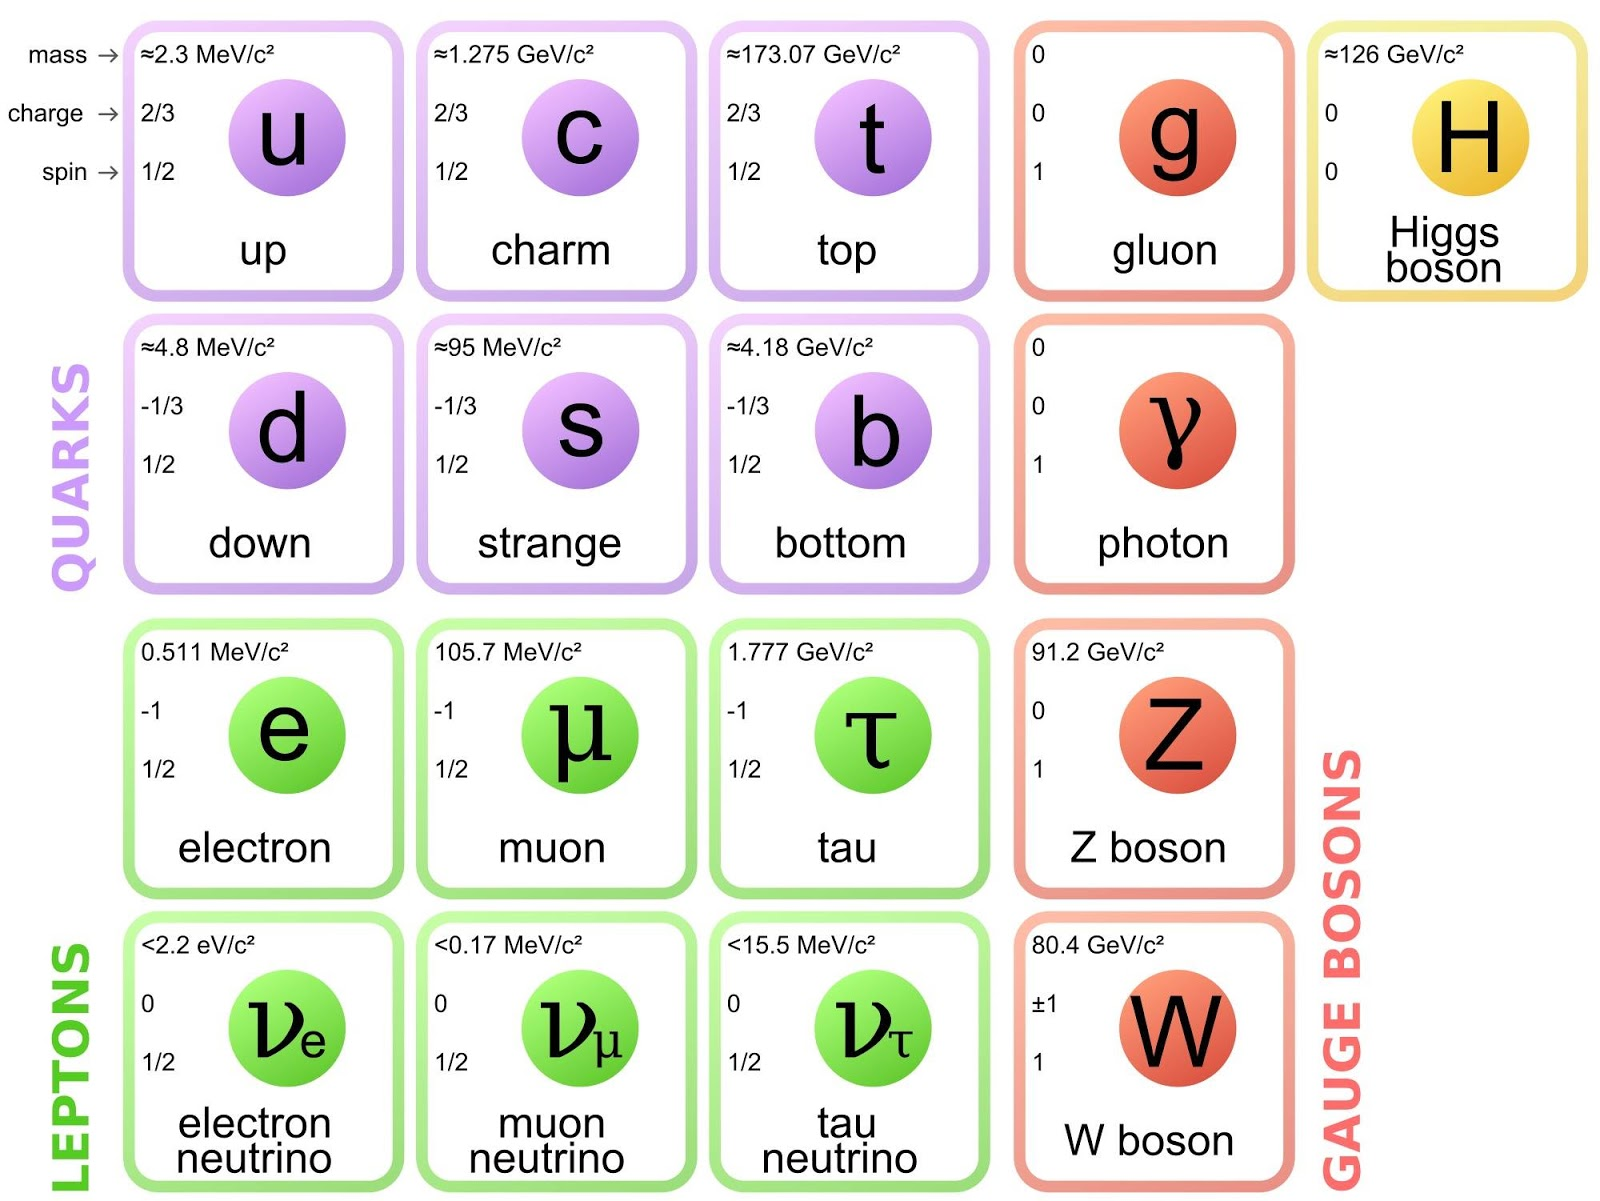
\includegraphics[width=.65\textwidth]{figures/standard-model.jpg}
  \caption{The fundamental particles posited by the Standard Model.}
  \label{fig:standard-model}
\end{figure}


The Lagrangian of QCD is given by
\begin{equation}
  \label{eqn:qcd-lagrangian}  
  \mathcal{L}_{\text{QCD}} = \sum_q \bar{\psi}_{q,a} \left( i\gamma^\mu \partial_\mu \delta_{ab} - g_s \gamma^\mu t_{ab}^{C} A_{\mu}^C - m_q \delta_{ab}\right)\psi_{q,b} - \frac{1}{4}F_{\mu\nu}^{A} F^{A\mu\nu}
\end{equation}
where pairs of indices are summed over and $\delta_{ab}$ is the Dirac delta operator.
The $\gamma^\mu$ are the Dirac $\gamma$-matrices, which embed spin dynamics of fermions.
The $\psi_{q,a}$ are quark fields for a quark of flavor $q$, mass $m_q$, and color-index $a$ (which runs from 1 to $N_C = 3$).
The $A_\mu^C$ represent the gluon fields, with the index $C$ running from 1 to $N_C^2 -1 = 8$, meaning there are 8 types of gluons.
The $t_{ab}^C$ are the generators of the SU(3) group (the Gell-Mann matrices), and correspond to 3$\times$3 matrices which embed the color dynamics on the quark/gluon interaction, and represent how gluons rotate the color state of an interacting quark.
The gluon field tensor $F^{A}_{\mu\nu}$ is given by
\begin{equation}
  \label{eqn:gluon-field-tensor}
  F_{\mu\nu}^A = \partial_\mu \mathcal{A}_\nu^A - \partial_\nu \mathcal{A}_\mu^A - g_s f_{ABC} \mathcal{A}_\mu^B \mathcal{A}_\nu^C
\end{equation}
where $f_{ABC}$ are the structure constants of SU(3) and are defined by the commutation relation $[t^A,t^B] = if_{ABC}t^C$.
The quantity $g_s = \sqrt{4\pi\alpha_s}$ is the \gls{qcd} coupling constant. The coupling constant and the quark masses are the only free parameters of \gls{qcd}.
Note that the third term \ref{eqn:gluon-field-tensor} distinguishes \gls{qcd} (the strong interaction), from \gls{qed}.
This term gives rise to the triplet and quartic gluon self-interaction terms, which can be seen in the Feynman diagrams of \gls{qcd} shown in \ref{fig:feynman-diagrams}.
The self-interactions can also be understood as a consequence of the gluon simultaneously carrying color charge while also transmitting the color-charge interactions.
The physical implications of these self-interactions are profound. 


\begin{figure}[ht]
  \begin{subfigure}{0.3\textwidth}
    \resizebox{\linewidth}{!}{
      \begin{tikzpicture}
        \begin{feynman}
          \vertex (a) {\( q \)};
          \vertex[below right=of a] (b);
          \vertex[below left=of b] (c) {\( q \)};
          \vertex[right=of b] (d) {\( g \)};
          \diagram*{
            (a) -- [fermion] (b),
            (b) -- [fermion] (c),
            (b) -- [gluon] (d),
          };
        \end{feynman}
      \end{tikzpicture}
    }
  \end{subfigure}
  \begin{subfigure}{0.3\textwidth}
    \resizebox{\linewidth}{!}{
      \begin{tikzpicture}
        \begin{feynman}
          \vertex (a) {\( g \)};
          \vertex[below right=of a] (b) ;
          \vertex[below left=of b] (c) {\( g \)};
          \vertex[right=of b] (d) {\( g \)};
          \diagram*{
            (a) -- [gluon] (b),
            (b) -- [gluon] (c),
            (b) -- [gluon] (d),
          };
        \end{feynman}
      \end{tikzpicture}
    }
  \end{subfigure}
  \begin{subfigure}{0.3\textwidth}
    \resizebox{\linewidth}{!}{
      \begin{tikzpicture}
      \begin{feynman}
        \vertex (a) {\( g \)};
        \vertex[below right=of a] (b) ;
        \vertex[below left=of b] (c) {\( g \)};
        \vertex[above right=of b] (d) {\( g \)};
        \vertex[below right=of b] (e) {\( g \)};
        \diagram*{
          (a) -- [gluon] (b),
          (b) -- [gluon] (c),
          (b) -- [gluon] (d),
          (b) -- [gluon] (e),
        };
      \end{feynman}
    \end{tikzpicture}
    }
  \end{subfigure}
  \caption{Feynman diagrams for the fundamental interaction vertices of QCD.}
  \label{fig:feynman-diagrams}
\end{figure}


Quarks and gluons are never observed in isolation: a phenomenon known as \textit{color confinement}.
They instead always form into color-neutral combinations, called hadrons.
Hadrons come in two types: baryons, which are quark triplet states, and mesons, which are quark doublet states.
This occurs because, for long-distance (low $Q^2$) interactions, the strong force coupling (given by $g_s$, or, equivalently, $\alpha_s$) is strong.
The reason for this phenomena is not immediately intuitive, and stems from the renormalization scheme for $\alpha_s$.
The running coupling of the strong interaction strength $\alpha_s$ is derived from the renormlization group equation
\begin{equation}
  \label{eqn:RGE}
  Q^2 \cfrac{\partial \alpha_s}{\partial Q^2} = \beta(\alpha_s)
\end{equation}
where the QCD $\beta$-function has the following perturbative expansion:
\begin{equation}
  \label{eqn:beta-function}
  \beta(\alpha_s) = -b \alpha_s^2 \left[1 + b'\alpha_s + b''\alpha_s^2  + O(\alpha_s^3)\right]
\end{equation}
where the coefficients $b$, $b'$, and $b''$ are found from the 1, 2, and 3-loop vacuum polarization contributions to the bare \gls{qcd} interaction vertex, respectively \cite{Ellis_Stirling_Webber_1996}.
If we only keep the lowest order term, \ref{eqn:RGE} becomes
\begin{equation}
  \label{eqn:RGE-lowest-order}
  Q^2 \cfrac{\partial \alpha_s}{\partial Q^2} \approx -b \alpha_s^2
\end{equation}
which has the solution
\begin{equation}
  \label{eqn:alpha-approx}
  \alpha_s \approx \cfrac{1}{b\ln\left(\frac{Q^2}{\Lambda^2}\right)}
\end{equation}
where $\Lambda$ comes from the choice of the constant of integration, and represents the scale at which the coupling will diverge.
The exact value for $\Lambda$ is definition-dependent -- the value will change depending on how many terms are kept in \ref{eqn:beta-function} and how many active quark flavors ($n_f$) are assumed.
For \gls{nlo} calculations with $n_f = 5$, $\Lambda$ is approximately 200 MeV.
Near the mass scale of light hadrons ($Q \sim 1$ GeV), $\alpha_s$ is large, which leads to the confinement of quarks and gluons inside hadrons.

As can be seen in \ref{eqn:alpha-approx}, high interaction energies (large $Q^2$), $\alpha_s$ becomes small.
At high enough $Q^2$, quarks and gluons can be completely liberated from their hadronic bonds.
This phenomenon is known as \textit{asymptotic freedom}.
Asymptotic freedom is an experimentally verified phenomenon: there exists many measurements of the \gls{qcd} coupling constant across a wide range of energies.
Because $\alpha_s$ is one of only a few free parameters of the Standard Model, it can be determined via many observables.
Experimental measurements of $\alpha_s$ are shown to agree with theory, as can be seen in \ref{fig:running-coupling} \cite{ParticleDataGroup:2024cfk}.

\begin{figure}[ht]
  \centering
  % Use .5\textwidth to only have the table fill half the page,
  % and \textwidth for the full page
  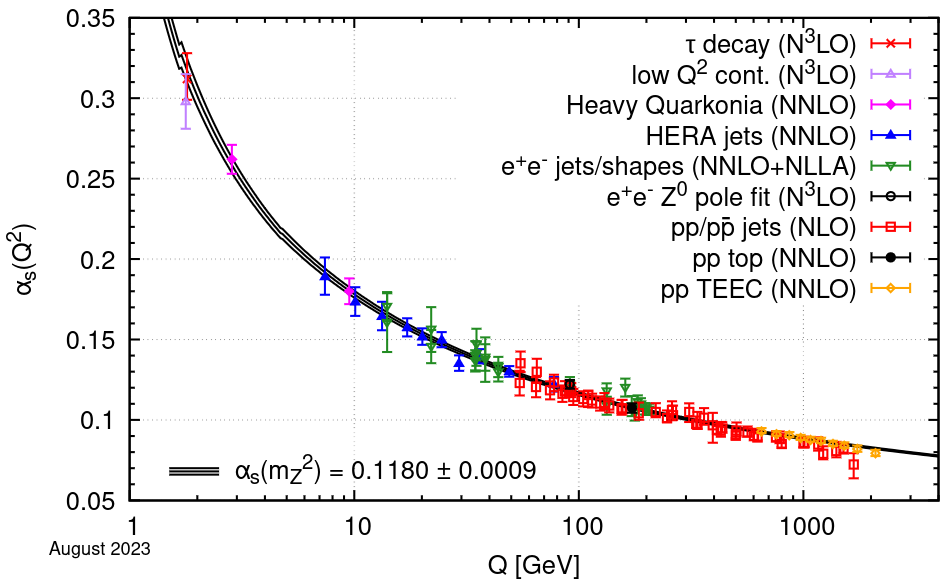
\includegraphics[width=.65\textwidth]{figures/running-coupling.png}
  \caption{Experimental measurements of the strong coupling strength $\alpha_s$ \protect\cite{ParticleDataGroup:2024cfk}.}
  \label{fig:running-coupling}
\end{figure}
%  Taken from \cite{ParticleDataGroup:2024cfk}









